\documentclass[10pt]{article}

\usepackage{arxiv}
\usepackage[utf8]{inputenc} % allow utf-8 input
\usepackage[T1]{fontenc}    % use 8-bit T1 fonts
\usepackage{hyperref}       % hyperlinks
\usepackage{url}            % simple URL typesetting
\usepackage{booktabs}       % professional-quality tables
\usepackage{amsfonts,amsbsy}       % blackboard math symbols
%\usepackage{nicefrac}       % compact symbols for 1/2, etc.
\usepackage{microtype}      % microtypography
\usepackage{graphicx, listings}
\usepackage{subcaption}
\usepackage{lipsum}
%\usepackage[sorting=ydnt]{biblatex}

\setlength{\parskip}{10mm}

\newcommand{\chembl}{\texttt{ChEMBL}}

\title{Deep Learning Techniques for the Prediction of Drug Target Interactions on a Kinome-wide Scale}

\author{
	\Large{Georgios Kalantzis}   \vspace{3mm} \\
	Department of Statistics and Doctoral Training Centre\\
	University of Oxford\\
	\texttt{georgios.kalantzis@seh.ox.ac.uk} \vspace{8mm}\\
	\textit{Supervised by Prof. Garrett Morris}\\
	\textit{In collaboration with Thierry Hanser, Lhasa Ltd Leeds}\\
%% Coauthor \\
%% Affiliation \\
%% Address \\
%% \texttt{email} \\
}

\begin{document}
\maketitle
\clearpage
\begin{center}
	\thispagestyle{empty}
	\vspace*{\fill}
	\begin{flushright}
		\textit{``All generalizations are dangerous. Even this one.''}\\
	 	Alexandre Dumas
	\end{flushright}
	\vspace*{\fill}
\end{center}
\newpage
\begin{abstract}
    \lipsum[1-2]
\end{abstract}

% keywords can be removed
%\tableofcontents
\vspace{1cm}
\keywords{Drug Target Interactions \and bioactivity prediction \and QSAR \and regression \and ChEMBL \and IC50 \and machine learning \and neural networks \and Multi-Task Learning \and matrix completion}

\clearpage
\section{Introduction}
Drug discovery is a long, challenging and expensive process that incorporates specialised knowledge from Medicine, Biochemistry and Pharmacology. Despite the advances in each of these fields, releasing a new drug to the market could cost up to 1.8 billion US dollars and require 13 years on average~\cite{rifaioglu2018recent}. To reduce this complexity, many computational methods have been developed during the last decades for virtual screening or computer-aided drug-design. These methods became effective with the advent of large databases with experimental data and the revolutionary applications of Machine Learning in every scientific domain. 

More than 20 thousand proteins exist in the human proteome and every pharmaceutical company retains libraries with millions of compounds, some of which could act as drugs dealing with a specific pathogenicity. This creates a space with billions of potential interactions between targets and compounds which the aforementioned databases aim to describe \cite{rifaioglu2018recent,gaulton2011chembl,bento2014chembl}. Aggregating the results by all the assays that have ever been conducted covers nothing but a small fraction of the total area.  Although the vast majority would not offer anything new, among all these interactions some are effective meaning that a compound can bind to a protein and activate the biological pathway for a desired effect. It is hypothesized that new drugs are still hidden somewhere in that space waiting to be discovered.

This project aims at exploring the use of various computational methods, including but not restricted to deep neural networks, for predicting the binding affinity of drug-target interactions (DTI). We will use data from ChEMBL, a publicly available database with protein-ligand binding information, and deploy common techniques for regression. We will investigate the effectiveness of methods that are known to work accurately, like random forests, and implement specialised techniques, like multi-task learning, to bypass specific bottlenecks. Our study is kinome-wide as we will design a framework to deal with hundreds of proteins from the family of kinases. Assuming that all the available data are placed in a drug-target table, we aim at imputing new values at the initially sparse matrix, a problem that can be described as \textit{matrix completion}. One way to tackle this is using non-negative matrix factorization and convex optimisation, techniques that do not require any features. In our case, however, interactions are accompanied by rich data that concern both targets and compounds. We will follow a compound-based approach and use chemical fingerprints as the only set of features.  
% and it is common in various scientific fields, like Recommender Systems. 

For the sake of this project we will use the terms \textit{drugs} and \textit{compounds} interchangeably, as well as \textit{proteins} and \textit{targets}. The rest of this report is structured as follows: Section~\ref{ss:relatedwork} gives a short review on the related literature, followed by an extensive description of our approach in Section~\ref{s:methods}. Then, Section~\ref{s:experiments} presents the design and the results of a variety of the computational experiments we conducted. Our study is finalised with a few conclusions in Section~\ref{ss:conclusions} and some snippets of code in the Appendix. 

%\clearpage
%\section{Background}

% \subsection{Problem definition and notation}


\section{Related Work}
\label{ss:relatedwork}


In general, published works on DTI could be divided in two broad categories, those studying classification and those on regression. For the first family of approaches, a bioactivity is classified as active or inactive according to whether the compound binds effectively on the target or not. Researchers can use a variety of thresholds (depending on which target or type of assay) to transform a measurement to 1 or 0, indicating an active compound or a decoy respectively. For the second family of methods, a regression algorithm is utilised for predicting the exact value of the binding between a target and a compound. For both cases, a variety of computational tools have been developed ranging from partial least squares to support vector machines or deep neural networks. We continue our analysis with reviewing a few such approaches that were recently published.  

%While regression is more challenging, it offers many advantages On the other hand, 

The biggest advantage of viewing the problem as a classification task is the ability of modelling interactions with many ways, one of that being the probabilistic matrix factorisation ~\cite{cobanoglu2013predicting}. This approach is purely quantitative as the only input is the binary connectivity matrix $\mathbf{R}_{N\times M}$ which is factorized by two matrices,  $\mathbf{U}_{N\times D}^\top$ and  $\mathbf{V}_{D\times M}$, that express drug-drug and target-target correlations in terms of $D$ latent variables. A probabilistic linear model with Gaussian noise is used to model interactions and matrices  $\mathbf{U}$ and $\mathbf{V}$ are such that a log-likelihood function is maximized, under constraints for failing to capture known interactions. Such a technique inherits the advantages of Collaborative Filtering~\cite{sarwar2001item}, since every compound is represented by the targets with which it interacts and compounds with similar representations ought to have similar chemical properties. 

To validate the intuition behind and the efficacy of this model, the authors of~\cite{cobanoglu2013predicting} run two sets of experiments. Firstly, they cluster the drugs within the latent space and compare the corresponding partition with that obtained by checking chemical or structural similarities. In brief, drugs that share common activities (i.e. lie close to each other in the latent space) do share common chemical characteristics for the majority of the cases. The next experiment of this study concerns the ability of the model to predict new interactions. By adopting a 5-fold cross-validation (and repeating for 100 times) they produce predictions, independently for four target types, and compare against two other published methods. They also compare a standard with an active learning version of the model by hiding $70\%$ of the dataset and incrementing it iteratively. In brief, the active learner is $1.44$ times more accurate than the passive learner and also better than other methods in the majority of the targets; performance varies from $0.650$ to $0.904$. 
%The data used are from DrugBank, versions of Sept 2011 and Sept 2013.

Neural networks constitute a common technique in Cheminformatics \cite{lecun2015deep,lenselink2017beyond,colwell2018statistical} where publicly available data sets constantly grow in sizes. Normally one would need to train a single model per target, thus the broader a study is with respect to the number of proteins studied, the longer training-time will need. However, \cite{ramsundar2015massively} is a promising approach that uses multi-task neural networks to predict novel interactions after training one model on an ensemble of data. The idea for using one ``big'' model instead of many ``small'' comes from the fact that single-task models use the same input (same set of features) and produce similar results. According to the authors, the most accurate approach is a pyramidal network with a wide shared layer to process the input, attached to a number of short layers, independently, which are then followed by a \textit{tanh} activation function.  

Another recent application of neural networks for regressing drug-target binding affinity is \cite{whitehead2019imputation}. The authors present a network that uses 320 chemical descriptors and sparse bioactivity data to predict novel $\texttt{pIC}_{50}$ values. They use a rather shallow neural network with one hidden layer and an iterative tool to impute missing values and sequentially expand the training data with the most accurate predictions. The missing values are initially replaced by the averages of the known values for each assay and then they are computed iteratively as 
\[ \mathbf{x}^{n+1} = \frac{\mathbf{x}^n + f(\mathbf{x}^n) }{2}. \]
Uncertainty is estimated by using an ensemble of twelve similar networks and hyperparameters for the NN architecture were selected after a random holdout validation. Deep learning techniques for drug discovery have met many more publications and a more detailed review can be found in~\cite{rifaioglu2018recent}.

%It is claimed that coefficient of determination could reach values higher than $0.90$ when using only the top-$1\%$ confident imputed data but the authors do not imply anything about the number of those predictions. 

%\subsection{Motivation}
To conclude, this field has gained a lot of attention and many approaches have been published. In order to offer some novelty, we will work on regression as the case of classification is densely studied. Our approach will be similar to that of \cite{martin2017profile} which, however, relies partially on private data and methods. The main contribution of the current study will be the application of multi-task learning for regression within the context of DTI. 

%\clearpage
\section{Data and Methods}
\label{s:methods}
In this section we describe the pipeline we created, in terms of data, features, and algorithms, for evaluating a method that accurately predicts new bioactivities. We give details only where is assumed as necessary and we skip the parameter selection for the next section. 


\subsection{The dataset}
\label{ss:dataset}

In order to use a curated data set, that is complete, robust and yet suitable for training methods and evaluating them fairly, we had to prepare one from scratch. To that end, we chose the latest version of \chembl, an online publibly available chemical database of bioactive molecules with drug-like properties~\cite{davies2015chembl,bento2014chembl,gaulton2011chembl}. While \chembl \ contains assay data from more than twelve thousand proteins, we focus only on kinases as they constitute an increasingly popular target for drug discovery because of their involvement in a wide range of pathological conditions. In particular, there are almost $800$ kinases in the database and fetching all the interactions for them resulted in a set with more than $800$ thousand activities; this is another indicator of the importance of this protein family in drug development. A summary of the total number of activities per type of measurement is shown in Fig.~\ref{fig:chembl}. We then selected those bioactivities measured with $IC50$, the inhibitory concentration at half-maximum, and filtered the data according to the following rules:
\begin{enumerate}
	\setlength\itemsep{0.5mm}
	\item Select compounds with SMILES representation so that we can calculate a fingerprints
	\item Remove questionably large values (there were cases with $\texttt{IC50} \geq 10000 nM$) 
	\item If there are many assays for the same drug-target pair, keep the one with the lowest value
	\item Select only those targets with at least $100$ interactions 
	\item Select only those compounds interacting with at least 2 targets.
\end{enumerate}

The last two steps were done iteratively as they depend on each other. At the end of this process, the data set was reduced to $110$ targets, $23,361$ compounds and a total of $62,656$ interactions. On average, there are $569.60$ interactions per target and $2.68$ per molecule. 

For a more qualitative point of view, we should have a look on the type of these bioactivities. A family-specific threshold for determining whether a compound binds effectively on a target or not is that of $30nM$\footnote{Check more at https://druggablegenome.net/ProteinFam}. Using that, $21,262$ interactions could be considered active, which is roughly one third of the entire data set; there is clearly a bias towards inactive compounds (or \textit{decoys}) as is common in virtual screening. Another important part of data preparation is the transformation to $-\log(\cdot)$ values, which is noted as \texttt{pIC50}. This offers some kind of rescaling which is important for regression and helps with reducing the impact of noise due to experimental inaccuracies. The corresponding distribution is showed in Fig.~\ref{fig:pic50}.

\begin{figure}
	\begin{subfigure}{.53\textwidth}
		\centering
		\caption{Kinases on \chembl}
		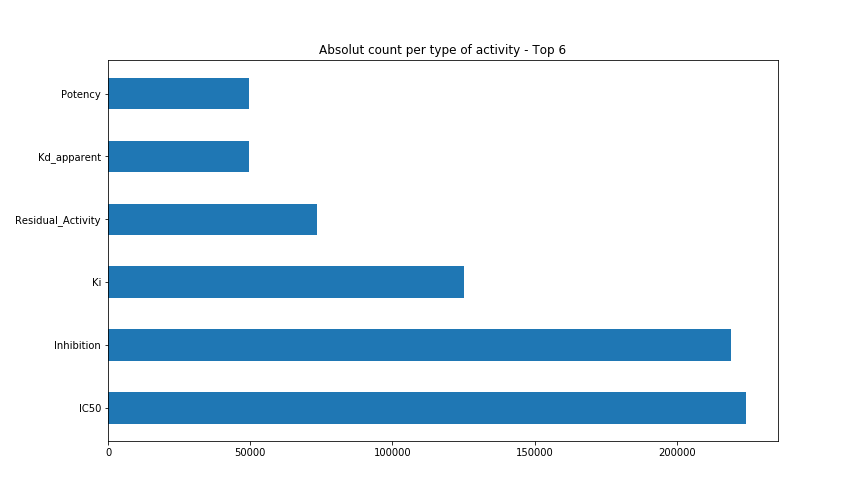
\includegraphics[width=\textwidth]{figs/activities-all.png}
		\label{fig:chembl}
	\end{subfigure}
	\begin{subfigure}{.53\textwidth}
%					\hspace{-10mm}
		\caption{Distribution of target variable} 
		\centering
		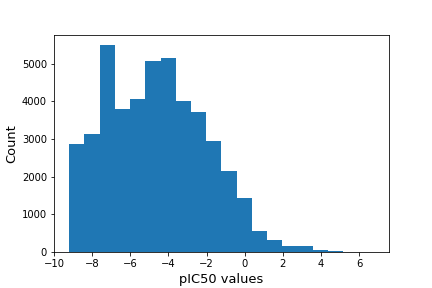
\includegraphics[width=\textwidth]{figs/TrueDistr.png}
		\label{fig:pic50}
	\end{subfigure}
\caption{{\small a) Absolute count of occurrences for each type of activity for the 797 kinases in \chembl. That's the \textit{initial} state of dataset. b) Distribution of the obtained \texttt{pIC50} values, the target-variable for the regression.} }
\end{figure}
 
\subsection{Features}
After selecting which targets to study, what type of data to use and which algorithm to rely on for predictions, the next thing to answer is what type of features should be used. Again, there are many options available, mainly categorised as chemical-similarity-based, target-similarity-based, or mixed. Due to repletion of the latter cases and time constraints set by the short duration of this project, we follow a compound-oriented approach by using chemical fingerprints as the only type of features for regression. 

Chemical fingerprints are a way of materialising compounds. A molecule is decomposed into a set of fragments, each centered at a non-hydrogen atom, which are then iteratively extended to neighboring atoms. Each fragment is assigned a unique identifier which are finally hashed into a fixed-length binary vector~\cite{ramsundar2015massively}. Such tools are commonly used in Cheminformatics, especially when there is a need of measuring similarity between compounds. We mainly work with extended connectivity fingerprints (ECFP4)  with $2048$ bits, which we calculated using \texttt{RDkit} and the function \texttt{GetMorganFingerprintAsBitVect} with radius $2$. 

\subsection{Single Task Learning as a baseline}

The first computational task of our project concerned the formation of a baseline with common techniques for regression in DTI. This baseline will be used as a reference for assessing the methods that will be implemented later on. A standard way for regression in the field relies on Random Forests (RF)~\cite{martin2017profile,whitehead2019imputation,colwell2018statistical}, which are an ensemble of single estimators (decision trees) with numerous advantages for many applications of machine learning. One reason, among others, that RF are commonly used by cheminformaticians is the feature selection process which they incorporate and which can be easily used for interpretation. 

When regression needs to be performed on high dimensional data, as with fingerprints, Lasso (LR)~\cite{tibshirani1996regression} is one reasonable tool. LR is a shrinkage method that performs both variable selection and regularisation in order to enhance the prediction accuracy and interpretability of the statistical model it produces. It uses a penalisation scheme with norm-1 which forces the coefficients of the linear model to act as ``binary'' objects that either have a meaningful value or are really close to zero.  An important feature of LR that makes it a convenient method is the only one parameter that needs optimisation, which is $\alpha$, the level of regularisation. 

Moreover, a third method that we are utilising in this stage are neural networks, an approach that has been proven to be accurate in many domains and that has recently gained tremendous amounts of attention, as we indicated in Section~\ref{ss:relatedwork}. A NN consists of many layers with nodes-weights for information processing. The first layer is applied directly to the input data, extracts some high level features which passes to the next hidden layer, and so on, until the final layer which ``produces'' the output; a real-value prediction for regression problems or a probability for classification. The more hidden layers a network has, the deeper it is. Non-linear functions are applied element-wise, between layers, on the information-flow; such functions are usually \textit{tanh, ReLU, softmax} which make NNs a non-linear method. Finally, there are types of architectures regarding the way information flows but for our purposes we study only fully connected networks; each node of one layer is connected to every node of the next layer.

For the application of RF, LR and NN we use the built-in implementations of Scikit-Learn \cite{scikit-learn},  Python's most famous module for machine learning. Parameters are selected after a quick grid-search with cross-validation; more details will be given at Section~\ref{SS:methodology}. Although it offers many methods and tools, Scikit-Learn was not enough for our needs  for NN in particular. Keras~\cite{chollet2015keras}, on the other hand, is a library specialised for deep learning which offers the ability to define every detail of the model's architecture and training process. Thus, we deploy a fourth  STL method, labelled as \texttt{myNN}, which is a NN with two hidden layers of 200 and 20 nodes respectively -- sizes that were selected by hand for a simple yet accurate model -- and a third layer with a single node for predictions. We use \texttt{tanh} as activation for the two hidden layers since this function has a wide range of output, something that is useful for dealing with \texttt{pIC50} values. Activation for the last layer is done with the identical function to keep the model simple. The parameter that we select by cross-validation is the level of regularisation for the weights of each layer.
%single task learning

%Network architecture is probably the most important parameter to fix for a NN and we select one among  models consisting of a few short hidden layers. 
%NN have recently and showed great performance but saying more is out of the scopes of this discussion.   Number of layers and activation function were selected 


\subsection{Multi Task Learning for a generalisation}

The approaches described in the previous section,  are \textit{single-task} (STL) since they require one model per target, i.e. we need to train 110 independent RF, 110 lasso regressors etc. Since all these models have the same input and similar output, one question that naturally arises is how we could design one model to capture the important features that are used and adapt them on each target individually; multi-task learning (MTL) is one answer. A multitask NN consists of a set of shared layers and a number of \textit{sub-networks} with hidden layers, one per task. The first part receives the input and extracts basic features, common for every task. Then, each of the sets with hidden layers is attached on parallel to the last shared layer and adapts the model to each target by extracting more special features. 

In brief, we deploy one larger NN, labelled as \texttt{MTL}, to deal with every task instead of many smaller models. Such a holistic approach is expected to make interpretation easier and offer a significant speed-up in training times. To be more precise, a MTL network needs to train $854,310$ parameters whereas 110 STL models require more than 22 million. Moreover, programming for the training and evaluation of a MTL method is by far easier, in terms or lines of code, than doing the same for 110 models. 

% TO DO: say more about computational benefits and GPU-CPU
% TO DO: talk about batch size - that should be "personalised" per STL model.

Similarly to what we used as a STL approach, we create a network with one shared layer and 110 subnetworks with one short layer (attached to the shared) followed by one single-node layer for predictions. Again, the activation functions between the layers are \texttt{tanh}. This time we select with cross-validation the level of regularisation as well as the sizes of the hidden layers.

\subsubsection{Drop-out}
% say more about overfitting ??
Recently, a probabilistic tool called \textit{drop-out} is widely used in deep NN as a regularisation step to avoid overfitting~\cite{ramsundar2015massively,lecun2015deep}. According to that, a node is randomly disregarded and the information from that is not passed to the next layer. It is usually expressed as a hyper-parameter of the model and a drop-rate of, e.g. $30\%$, between the first two layers means that roughly one-third of the nodes in the first layer will be dropped. Drop-out can be applied between any two layers or in combinations of pairs. As this can have a high effect in performance, drop-out needs to be careful selected. To that end, we will train another model, called \texttt{MTLD} and a similar to \texttt{MTL}, to assess the use of dropout in our problem.  \texttt{MTLD} will include a drop-out on the shared layer and a fixed kernel regularisation on the following layers. Thus, the parameters to select are the sizes of the hidden layers and the drop-rate.

\clearpage
\section{Experimental Evaluation}
\label{s:experiments}

In this section we will give answers to a series of questions regarding the performance of the aforementioned methods in the prediction of DTI. We start by describing the evaluation methodology that we follow, continue by assessing the STL methods and then investigate the advantages offered by MTL. We also explore the use of dropout and ways to enhance accuracy by self-training.

\subsection{Methodology}
\label{SS:methodology}
  
In order to achieve maximum transparency while training and fairness during evaluation, we partition the data set in three (disjoint) sets of interactions. Firstly, we randomly select  $3,132$ from the set of active interactions and the same number from the set of inactive, which in total is $10\%$ of the data, and form a test set that will be used for a final assessment. Then we randomly select $20\%$ of the remaining data (or $18\%$ of the whole dataset) for the validation set and the rest acts as training data. 
 
Using scikit's \texttt{GridSearchCV}, we follow a 4-fold cross-validation to select parameters for the STL methods through a quick grid search. We select those that have the highest average accuracy across the 4 folds, then fit each algorithm to the $80\%$ and evaluate with the validation set. For RF we search for the ideal number of trees among the numbers $[10,25,50,100,150,300]$ and the \textit{max depth} from $[10,100,200,500]$. For the case of NN, the unknown parameters are the number of hidden layers and the number of nodes within each. Since training one model for each target is an expensive procedure, we run a quick search among $[(50),(100,20),(100,50),(500,20,10)]$, which stand for one, two, two, and three hidden layers. The activation function is set to \textit{tanh}  and the selected solver is \textit{Limited-memory BFGS}. For the case of LR we search for the optimal level of regularisation among the values $[0.01,0.1,0.5,1]$. Similarly for \texttt{myNN}, we use the range $[0.001,0.01,0.1, 0.2]$ and train each model for 250 epochs, in batches of 20 (as some targets contain only a few dozens of observations) with a learning rate of $0.001$.

For the two MTL approaches, we use a variety of combinations for designing a model, namely the cartesian product of the sets $[2000,1000,300,200]$ for the shared layer, $[200,100,50,20]$ for the parallel hidden layers and $[0.02, 0.05, 0.1, 0.2]$ for regularisation or $[0.05, 0.1, 0.2]$ for the drop-out. One important difference between the STL versions and these models is that we have tens of thousands of observations available now. To keep training duration on reasonable levels, we use batches of 64 or 128 observations and 30-50 epochs.

Accuracy is measured with the coefficient of determination, a casual metric in regression, defined as 
\[ R^2 = 1 - \frac{ \sum (y_i - \hat{y}_i)^2 }{ \sum (y_i - \bar{y})^2}, \]
where $y_i$ is the true value, $\hat{y}_i$ is the corresponding prediction and the sum runs for all the observations of a target or for the whole validation set. $R^2$ can get a maximum of $1.0$, indicating a perfect fit, and arbitrarily negative values when prediction is poor. In some cases we also use the mean squared error (MSE), which is also very common. 

%\subsection{Results}

\subsection{Results on Single Task Learning}
On a target-wise perspective, Fig.~\ref{fig:train} gives some insight on the performance during training for each of the four STL methods. The two NN approaches achieve a great fit to the data, confirming what is common experience for such methods. RF comes next with a quite robust accuracy of $\sim 0.8960$ on average and last is the LR which presents high oscillations, with an average of  $0.7524$ and a clearly decreasing motif as the size of training set is increased. 

Nevertheless, things are quite different when it comes for validation, as Fig.~\ref{fig:valid} indicates. RF outperforms every other method with an average $R^2$ of $ 0.5023$, and a st.d. of $0.1691$. NN approaches seem to overfit the training data as their accuracy has a significant decrease on the validation set. In particular, \texttt{myNN} comes second with a score of $0.4502$ and then is LR which achieves higher accuracy ($0.4190$) on average than the \texttt{skNN} ($0.3872$) but still low. The st.d. is $0.2162, 0.2135$ and $0.2648$ for \texttt{myNN}, \texttt{LR} and \texttt{skNN} respectively. One reason that all the methods seem unable to generalise effectively is the existence of a few outliers; there are a few cases for which they all fail dramatically, getting a very low $R^2$ which pulls the average score down. 

The results are more positive on an interaction-wise perspective, i.e. averaging for every point in the validation set. Ranking stays the same and the average $R^2$ scores are $0.648743, 0.625272, 0.5911$ and  $0.5826$ for \texttt{RF}, \texttt{myNN}, \texttt{LR} and \texttt{skNN} respectively. This means that the outliers are minor and manage to get hidden among a large set of quite good predictions. There  is one quick conclusion after comparing the two NN approaches about the importance of designing an effective model. NNs are prone to overfitting; they can clearly capture perfectly what is expressed in the training data but need careful parametrisation in order to generalise accurately. More comments are given in Section~\ref{ss:conclusions}.

\begin{figure}
	\begin{subfigure}{.53\textwidth}
		\centering
		\caption{Training accuracy}
		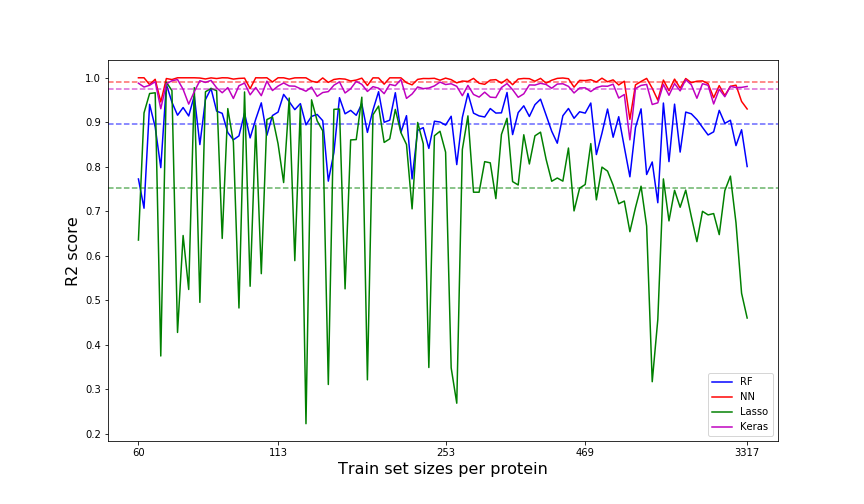
\includegraphics[width=\textwidth]{figs/Train-all.png}
		\label{fig:train}
	\end{subfigure}
	\begin{subfigure}{.53\textwidth}
%					\hspace{-10mm}
		\caption{Validation accuracy}
		\centering
		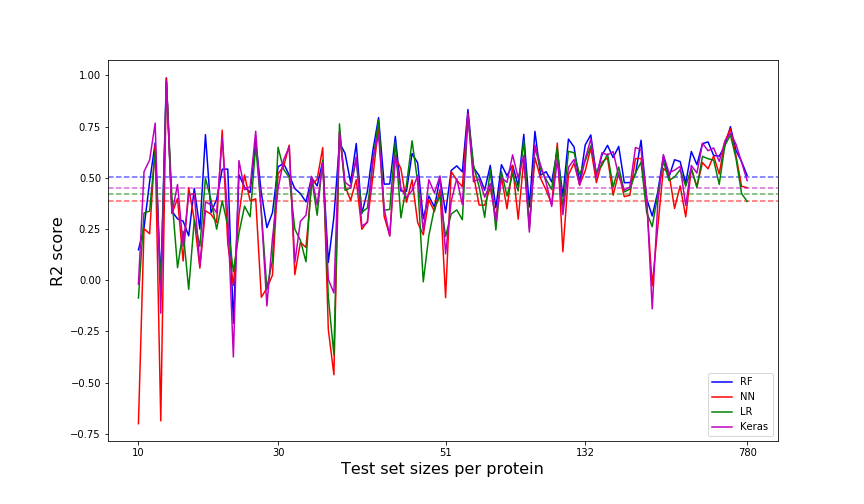
\includegraphics[width=\textwidth]{figs/Valid-all.png}
		\label{fig:valid}
	\end{subfigure}
\caption{{\small a) $R^2$ score after fitting on the training data. Horizontal lines indicate the average performance across the 110 targets, after selecting the best parametrisation with CV.  b) As in (a) but for the validation set.}}
\end{figure}


\subsection{Results on Multi Task Learning}

We proceed with the experiments about the advantages of MTL. As indicated earlier, this model ought to be different than the ``optimal'' STL version and it took us many trials to come up with an effective architecture. Training took place using masked mean squared error as a loss function which is a way to omit the missing values and calculate the divergence of the predictions from the true values only for the training points. After fitting a variety of models in the training set -- as described in a previous paragraph -- we selected as optimal parametrisation the one with the maximum mean performance, i.e. the minimum average MSE. 

For the \texttt{MTLD}, the winning setting consisted of 200 nodes for the shared layer, 20 for each of the parallel and $0.02$ for regularisation, trained with a learning rate equal to $0.0001$, 50 epochs and batches of 128 observations. 

Figures ~\ref{fig:MTL} and \ref{fig:MTLD} are similar to that of ~\ref{fig:valid}, after grouping the predictions for each target. Despite the fact that \texttt{MTLD} does not behave well enough, \texttt{MTL} achieves an accuracy similar to that of the STL approaches (mean $R^2 = 0.5600$ with st.d.$=9990$); Moreover, averaging across the validation set, \texttt{MTL} and \texttt{MTLD} have a mean $R^2$ of $9999$ and $999$ respectively, with a st.d. of $999$ and $999$. This is a surprising result as it indicates the effectiveness of multi-task models. In addition, training \texttt{MTL} would last roughly 18 minutes on average whereas training 110 STL models took almost the double. MTL is beneficial both in terms of efficiency and accuracy. 

\begin{figure}[h]
	\begin{subfigure}{.53\textwidth}
		\centering
		\caption{TO DO - MTL model}
		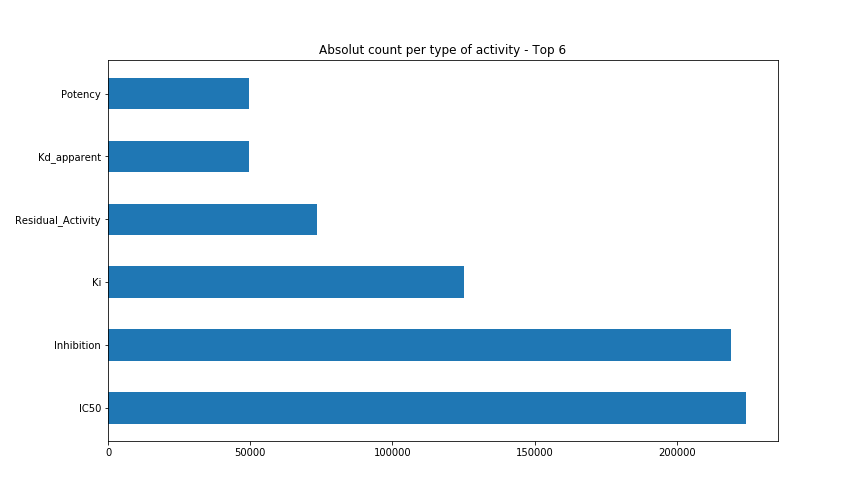
\includegraphics[width=\textwidth]{figs/activities-all.png}
		\label{fig:MTL}
	\end{subfigure}
	\begin{subfigure}{.53\textwidth}
		%					\hspace{-10mm}
		\caption{TO DO - MTL with dropout} 
		\centering
		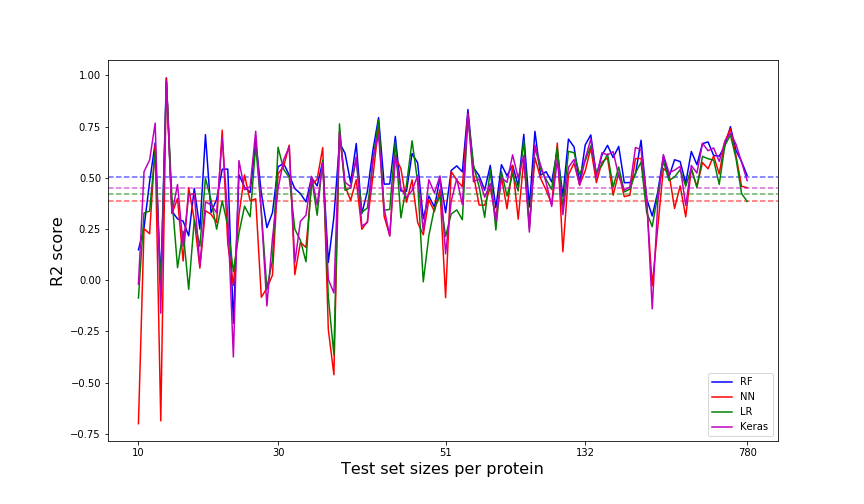
\includegraphics[width=\textwidth]{figs/Valid-all.png}
		\label{fig:MTLD}
	\end{subfigure}
	\caption{{\small  TO-DO. Performance for various lengths of training time. As the number of iterations is increased, each model is adapted better to the data but the ability to generalise is slightly decreased.} }
\end{figure}

\subsection{Self-training for an improvement}

Another experiment concerns the impact of iteratively expanding the training set with confident predictions. This is essentially the ability of a model to self-train itself in order to become more accurate. The essential tool for self-training is the complement of a prediction with a level of uncertainty/confidence. There are many techniques to do this, either by modifying the existing method, like adding some type of noise, or by producing multiple copies of the same procedure, like training many models on different subsets of the train set. In any case, each prediction would be an ensemble of the occurring values and uncertainty could be estimated by the volume of variance or the width of a confidence interval.   

Random forests offer a direct way of producing different estimations of one prediction. They work as an ensemble of decision trees by averaging the individual predictions. Each decision tree acts as an estimator of the prediction and analysing these values can provide the desired confidence. Using the RF models that were trained for the previous task, we will assess their potential to become even more accurate. There is a serious drawback for this procedure which lies in the nature of STL; we need to run the aforementioned cycle for all the 110 targets.

On the other hand, \texttt{MTLD} can bypass this bottleneck. But how could we assess how much confident the NN is for a single prediction? Whitehead et al.~\cite{whitehead2019imputation} train twelve separate networks and use the corresponding variance as a level of uncertainty; they claim that this methodology is advantageous as they manage to increase the accuracy of their model. As we think that such an approach loses in efficiency, we turn our attention on drop-out and the seminal work of Gal et al.~\cite{gal2016dropout} for uncertainty in deep learning. During the testing phase, drop-out makes the model stochastic. Repetitive runs with the same input will make different nodes drop, thus the output will be a sum of different weights. Provided the model has converged, the diversity of predictions for the same input should be small.

For the two approaches, we examine the width of a $95\%$ confidence interval for each prediction and use a threshold to discriminate the confident from the unreliable cases. We impute the first in the dataset, re-train each model and repeat until no more predictions are confident or until we have a large number of training data. The results are unfortunate for the RF but promising for \texttt{MTLD}. RF, no matter the threshold, stay on the same levels of accuracy or behave even worse. On the contrary, \texttt{MTLD} manages to get a minor improvement in most of the cases.  

\subsection{Final evaluation}
Our final computational task simulates a realistic application where we are asked to extrapolate, i.e. impute the missing values of the so-called DTI matrix. Practically, when an algorithm is in action and predicts the potency between a ligand and a protein, there is no way to assess unless someone runs the corresponding assay. That is the role of the test set that we initially crated. Normally we should apply only one method -- the one that would be our model-answer to deal with the problem -- but, as our project aims at exploring a variety of techniques, we will apply the \texttt{RF}, \texttt{MTL} and \texttt{MTLD} (the leading methods for each of the previous parts), on the $90\%$ of the data set that is not hidden.

Interestingly, the results are similar to those for the validation set indicating that each method is robust enough to generalise. In particular, \texttt{RF} obtained an accuracy of $0.6765$ and \texttt{MTL} comes next with $0.5953$, values which are averaged across the test set. On a target-wise perspective, RF had an average of $0.5263$ versus $0.3468$ for the \texttt{MTL}. Self training obtained similar levels of accuracy, as well. Another type of comparison  for these methods is depicted in fig.~\ref{fig:test} which shows the obtained distributions. 

\begin{figure}[h]
	\begin{minipage}[c]{0.6\textwidth}
		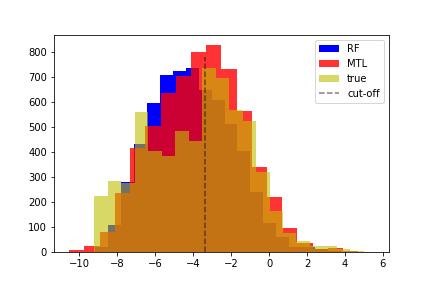
\includegraphics[width=\textwidth]{figs/Distr-Testset.png}
	\end{minipage}\hfill
	\begin{minipage}[c]{0.38\textwidth}
		\caption{{\small Comparison of the prediction-distribution for each method depicted along with the distribution of the true values. The dashed line indicates the threshold used to discriminate between active and decoys. The right part of the figure corresponds to the true positives and both methods behave quite well. For the decoys however, which are probably more diverse, there are more inaccuracies. }} 	
		\label{fig:test}
	\end{minipage}
\end{figure}


%\clearpage
\section{Conclusions}
\label{ss:conclusions}

We completed a detailed investigation of methods for regressing the binding affinity between compounds and targets. Our project involved the use of chemical fingerprints as the only feature for predicting \texttt{pIC50} values, a problem that, to the best of our knowledge, was not studied before in this form. The outcomes of our experiments made clear that the problem is tractable and maybe even solvable, since every method could be further optimised.
 
It was clear that random forests and neural networks are more suitable for single targets but for analysing more proteins, like a kinome-wide study, multi-task models provide more advantages. They offer a speed up during training, simpler pipeline implementation and can achieve equally good performance.

% profiling  

\subsection{Future work}

Throughout our study, we worked with fully connected neural networks, which is maybe the simplest form of deep learning. Thus one could increase accuracy with more complicated models like CNN or LSTM. The same holds for the case of random forests for which our optimisation could have been more careful and there are improved algorithms available (XGBoost), as well.

We noticed similar results while using a different type of fingerprints, the feature-based (FCFP) but details are skipped due to space restrictions. Thus, one direction worth exploring more is to find out which type, and why, offers more information. Moreover, we believe it is possible to unmask important features with reverse-engineering. For instance, fig.~\ref{fig:features} shows the existence of only a few bits with high impact on regression. 
\begin{figure}[h]
    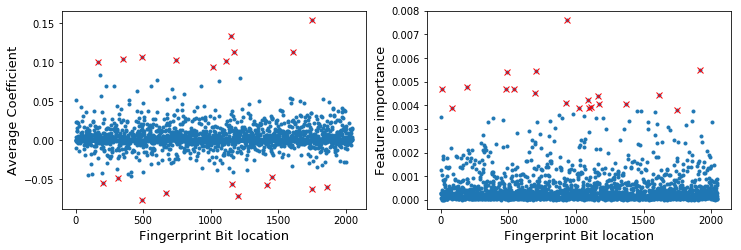
\includegraphics[width=\textwidth]{figs/FP-bits.png}
	\caption{{\small Left: Coefficients for ECFP bits obtained by LR, averaged for all target-models. Right: Importance of features obtained by analysing RF models. In both cases, the vast majority is close to zero except some with consistently larger values, which are shown with crosses.}}
	\label{fig:features}
\end{figure}

Finally, another interesting extension of this project would be the application of our methods on another dataset. Either to a different set of proteins (like GPCRs) or to a popular data set, like the one with 159 assays~\cite{martin2017profile}. The latter would make easy the comparison of our best method with other previously published techniques. 
%\subsection{Application on the ``realistic dataset''}

\clearpage
\bibliographystyle{ieeetr}  
\bibliography{project2_references}
\end{document}